\iffalse
\documentclass[]{article}
\usepackage{amsfonts, amssymb}
\usepackage{amsmath}
\usepackage{amsthm}
\usepackage{mathtools}
\usepackage{algorithmic}
\usepackage{float}
\usepackage{graphicx}
\usepackage{enumitem}

\newtheorem{theorem}{Theorem}[section]
\newtheorem{problem}{Problem}
\newtheorem{proposition}{Proposition}[section]
\newtheorem{lemma}{Lemma}[section]
\newtheorem{corollary}[theorem]{Corollary}
\newtheorem{example}{Example}[section]
\newtheorem{definition}[problem]{Definition}
%\newtheorem{thm}{Theorem}[section] 
%\newtheorem{defn}[thm]{Definition}
%\newtheorem{algorithm}{Algorithm}[section]
%\newtheorem{cor}{Corollary}
\newcommand{\BEQA}{\begin{eqnarray}}
\newcommand{\EEQA}{\end{eqnarray}}
\newcommand{\define}{\stackrel{\triangle}{=}}
\theoremstyle{remark}
\newtheorem{rem}{Remark}
%\bibliographystyle{ieeetr}

\title{Question 39.2023}
\author{Anupama Kulshreshtha \\ EE22BTECH11009}
\date{}
\begin{document}
\maketitle
\providecommand{\pr}[1]{\ensuremath{\Pr\left(#1\right)}}
\providecommand{\prt}[2]{\ensuremath{p_{#1}^{\left(#2\right)} }}        % own macro for this question
\providecommand{\qfunc}[1]{\ensuremath{Q\left(#1\right)}}
\providecommand{\sbrak}[1]{\ensuremath{{}\left[#1\right]}}
\providecommand{\lsbrak}[1]{\ensuremath{{}\left[#1\right.}}
\providecommand{\rsbrak}[1]{\ensuremath{{}\left.#1\right]}}
\providecommand{\brak}[1]{\ensuremath{\left(#1\right)}}
\providecommand{\lbrak}[1]{\ensuremath{\left(#1\right.}}
\providecommand{\rbrak}[1]{\ensuremath{\left.#1\right)}}
\providecommand{\cbrak}[1]{\ensuremath{\left\{#1\right\}}}
\providecommand{\lcbrak}[1]{\ensuremath{\left\{#1\right.}}
\providecommand{\rcbrak}[1]{\ensuremath{\left.#1\right\}}}
\newcommand{\sgn}{\mathop{\mathrm{sgn}}}
\providecommand{\abs}[1]{\left\vert#1\right\vert}
\providecommand{\res}[1]{\Res\displaylimits_{#1}} 
\providecommand{\norm}[1]{\left\lVert#1\right\rVert}
%\providecommand{\norm}[1]{\lVert#1\rVert}
\providecommand{\mtx}[1]{\mathbf{#1}}
\providecommand{\mean}[1]{E\left[ #1 \right]}
\providecommand{\cond}[2]{#1\middle|#2}
\providecommand{\fourier}{\overset{\mathcal{F}}{ \rightleftharpoons}}
\newenvironment{amatrix}[1]{%
  \left(\begin{array}{@{}*{#1}{c}|c@{}}
}{%
  \end{array}\right)
}
%\providecommand{\hilbert}{\overset{\mathcal{H}}{ \rightleftharpoons}}
%\providecommand{\system}{\overset{\mathcal{H}}{ \longleftrightarrow}}
	%\newcommand{\solution}[2]{\textbf{Solution:}{#1}}
\newcommand{\solution}{\noindent \textbf{Solution: }}
\newcommand{\cosec}{\,\text{cosec}\,}
\providecommand{\dec}[2]{\ensuremath{\overset{#1}{\underset{#2}{\gtrless}}}}
\newcommand{\myvec}[1]{\ensuremath{\begin{pmatrix}#1\end{pmatrix}}}
\newcommand{\mydet}[1]{\ensuremath{\begin{vmatrix}#1\end{vmatrix}}}
\newcommand{\myaugvec}[2]{\ensuremath{\begin{amatrix}{#1}#2\end{amatrix}}}
\providecommand{\rank}{\text{rank}}
\providecommand{\pr}[1]{\ensuremath{\Pr\left(#1\right)}}
\providecommand{\qfunc}[1]{\ensuremath{Q\left(#1\right)}}
	\newcommand*{\permcomb}[4][0mu]{{{}^{#3}\mkern#1#2_{#4}}}
\newcommand*{\perm}[1][-3mu]{\permcomb[#1]{P}}
\newcommand*{\comb}[1][-1mu]{\permcomb[#1]{C}}
\providecommand{\qfunc}[1]{\ensuremath{Q\left(#1\right)}}
\providecommand{\gauss}[2]{\mathcal{N}\ensuremath{\left(#1,#2\right)}}
\providecommand{\diff}[2]{\ensuremath{\frac{d{#1}}{d{#2}}}}
\providecommand{\myceil}[1]{\left \lceil #1 \right \rceil }
\newcommand\figref{Fig.~\ref}
\newcommand\tabref{Table~\ref}
\newcommand{\sinc}{\,\text{sinc}\,}
\newcommand{\rect}{\,\text{rect}\,}
%%
%	%\newcommand{\solution}[2]{\textbf{Solution:}{#1}}
%\newcommand{\solution}{\noindent \textbf{Solution: }}
%\newcommand{\cosec}{\,\text{cosec}\,}
%\numberwithin{equation}{section}
%\numberwithin{equation}{subsection}
%\numberwithin{problem}{section}
%\numberwithin{definition}{section}
%\makeatletter
%\@addtoreset{figure}{problem}
%\makeatother

%\let\StandardTheFigure\thefigure
\let\vec\mathbf

Let $X_1$, $X_2$, ... , $X_n$ be a random sample of size $n$ from a population having probability density function
\begin{align}
p_X(x; \mu) =
\begin{cases}
e^{-(x-\mu)}, & \text{if } \mu \leq x < \infty \\
0, & \text{otherwise,} 
\end{cases}
\end{align}
where $\mu \in \mathbb{R}$ is an unknown parameter. If $\hat{M}$ is the maximum likelihood estimator of the median of $X_1$, then which one of the following statements is true?
\begin{enumerate}[label=\Alph*)]
  \item $\pr{\hat{M} \leq 2}$ = $1 - e^{-n(1-\log_e 2)}$ if $\mu = 1$
  \item $\pr{\hat{M} \leq 1}$ = $1 - e^{-n \log_e 2}$ if $\mu = 1$
  \item $\pr{\hat{M} \leq 3}$ = $1 - e^{-n(1-\log_e 2)}$ if $\mu = 1$
  \item $\pr{\hat{M} \leq 4}$ = $1 - e^{-n(2\log_e 2-1)}$ if $\mu = 1$
\end{enumerate}
\fi
\solution
For continuous random variable X, median M is such that,
\begin{align}
\pr{X \leq M} &= 0.5
\end{align}
The pdf of X is given by,
\begin{align}
p_X(x) =
\begin{cases}
e^{-(x-\mu)}, & \text{if } \mu \leq x < \infty \\
0, & \text{otherwise,} 
\end{cases}
\label{eq:391}
\end{align}
Hence, cdf is given by
\begin{align}
F_X(x; \mu) &= \int_{\mu}^{x} e^{-(t-\mu)}dt\\ 
&= e^{\mu}[-e^{-x} + e^{-\mu}]\\
&= 1 - e^{-(x-\mu)}
\end{align}
Now,
\begin{align}
F_X(x; \mu) &= 0.5\\
\implies 1 - e^{-(M-\mu)} &= 0.5\\
\implies \hat{M} &= \mu + \ln(2)
\label{eq:39}
\end{align}
\begin{definition}
L, the Maximum Likelihood Estimator of the distribution is given by,
\begin{align}
L &= \prod e^{-(x-\mu)}\\
&= e^{-(\sum x_i-n\mu)}\\
\end{align}
\end{definition}
For the Likelihood function to be maximum,
$\sum x_i-n\mu$ should be minimum
Hence,
\begin{align}
X_i > \mu\\
\implies \sum x_i > n\mu\\
\sum x_i-n\mu > 0\\
\implies \mu &= \frac{\sum x_i}{n}
\end{align}
Given,
\begin{align}
p_X(x) &= e^{-(x-\mu)}\\
\end{align}
$X_i$ follows an exponential distribution.
\begin{definition}
We know that if,
\begin{align}
p_X(x) &= \lambda_ie^{-\lambda_ix}\\
S &= X_1 + X_2 +..... +X_n\\
p_S(n) &= \frac{\lambda^nx^{n-1}e^{-\lambda x}}{(n-1)!}
\end{align}
which is gamma distribution with parameters n and $\lambda$
\end{definition}
Hence, pdf of 
\begin{align}
Y &= \sum_{i=1}^{n} x_i\\
\text{where,}\\
p_X(x) &= e^{-(x-\mu)}
\end{align}
will follow gamma distribution with parameter n and $\lambda = 1$, given by,
\begin{align}
p_Y(x;n,1) &= \frac{x^{n-1}e^{-x}}{(n-1)!}
\end{align}
Hence, cdf is given by,
\begin{align}
F_Y(x;n) &= \int_{1}^{x} \frac{t^{n-1}e^{-t}}{(n-1)!} \,dt \\
&= 1 - \Gamma(n,x)
\end{align}
where $\Gamma(n,x)$ is incomplete gamma function.
Thus,
\begin{align}
\pr{\hat{M} \leq k} &= \pr{\frac{\sum x_i}{n} + \ln(2) \leq k}\\
&= \pr{Y/n + \ln(2) \leq k}\\
&= \pr{Y \leq n(k - \ln(2))}\\
&= F_Y(n(k-\ln(2)))\\
&= 1 - \Gamma(n,n(k-ln2))
\end{align}
It needs a value of n to be computed.
\begin{figure}[htbp]
    \centering
    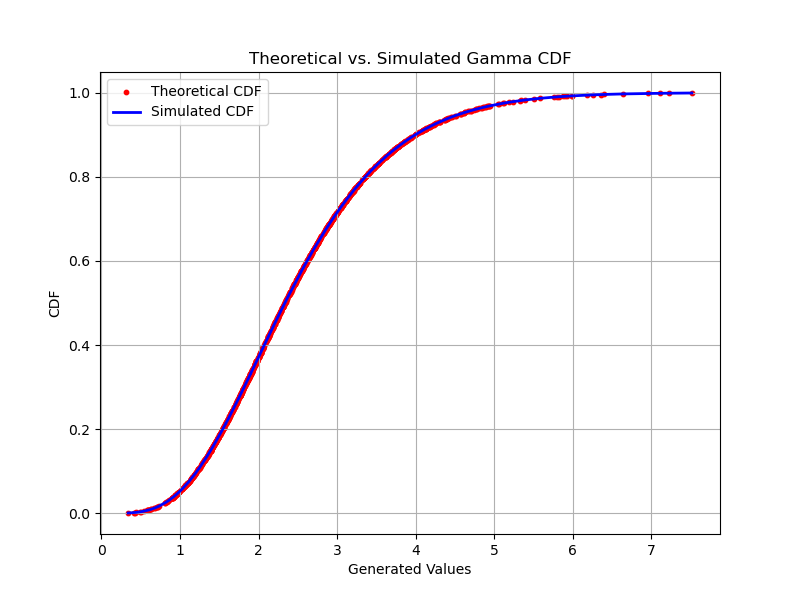
\includegraphics[width=0.8\textwidth]{2023/ST/39/figs/fig.png} 
    \caption{Verifying gamma cdf through simulation}
    \label{fig:39/2023}
\end{figure}\\
Steps for simulation in C:
\begin{enumerate}
\item Import the necessary libraries, including 'stdio.h','stdlib.h' and 'math.h'.
\item Write functions for generating exponential distribution, gamma pdf and gamma cdf.
\item In the main function, the exponentials generated using the function are added and stored in variable 'gamma samples' for each sample, to get sum of exponentials.
\item Then the simulated gamma cdf values are calculated using 'gamma cdf' function and the calculated sum of exponentials.
\item The code is then compiled using GCC compiler in the terminal (gcc simulation.c -o simulation -lm), and the results are stored in an output.txt file. (./simulation$>$output.txt)
\item The output file is loaded into the python code with theoretical cdf values, and the final graph between theoretical and simulated cdf is plotted.
\item The simulated and theoretical cdf values match, which verifies the gamma cdf through simulation.
\end{enumerate}
